% !TEX root = SystemTemplate.tex
\chapter{Design and Implementation}
The testing program has 6 main features which needed to be included.
These were:
\begin{enumerate}
	\item Finding the location of files containing existing test cases for the tested program to run
	\item Running the single program against the located test cases
	\item Recording and summarizing the test results
	\item Running test cases on entire class
	\item Running critical test cases separately from normal cases
	\item Creating test cases and corresponding answer files
\end{enumerate}
All features were written in C++ with each team members using their text
editors of choice.
\\ See the algorithm in algorithms~\ref{alg1} and ~\ref{alg2} below.
\begin{algorithm} [H] 
\caption{Automated Testing Program: Part 1}
\label{alg1}
\begin{algorithmic}    

\REQUIRE Program being tested from command line
\STATE Prompt for running or creating test cases
    \IF{Testing student cpp programs} 
        \ENSURE Test cases are found
        \IF{not in lowest level directory}
            \STATE Find .tst files in current directory
            \STATE Add file paths to .tst file to vector
            \STATE Drop into each subdirectory
        \ELSE
            \STATE Return to parent directory
        \ENDIF
        \ENSURE All students are found
        \IF{not in lowest level directory}
            \STATE Find .cpp files in current directory
            \IF{name.cpp equals parent directory name}
                \STATE Add file paths to student file to vector
            \ENDIF
            \STATE Drop into each subdirectory
        \ELSE
            \STATE Return to parent directory
        \ENDIF
        \ENSURE Test cases are run
        \STATE Compile C++ source code
        
        \WHILE{Not all students have been tested}
            \WHILE{not all test cases have been run}
                \STATE Run program against critical test cases
                \IF{Student didn't pass critical test cases}
                    \STATE Record that the student FAILED
                \ELSE
                    \STATE Run other test cases
                \ENDIF
                \STATE Record student results to student .log file
            \ENDWHILE
        \ENDWHILE
        \STATE Output main .log file with test statistics
    \ENDIF
\end{algorithmic}
\end{algorithm}
\pagebreak
\begin{algorithm} [H]
\caption{Automated Testing Program: Part 2}
\label{alg2}
\begin{algorithmic}
  
    \IF{Creating test cases}
        \STATE Prompt for number of test cases
        \STATE Prompt for number of entries in each test case
        \STATE Prompt if user wants to enter min file-entry value
        \IF{User wanted min value}
            \STATE Get min value
		\ENDIF        
        \STATE Prompt if user wants to enter max file-entry value
        \IF{User wanted max value}
            \STATE Get max value
        \ENDIF
        \STATE Prompt if user wants to enter test file name
        \IF{User wants custom test file names}
            \STATE Prompt for file name
		\ENDIF
        \WHILE{Not all test files have been created}
            \STATE Generate random file length L from 0 to File Max Length
            \WHILE{Less than L numbers have been written to file}
                \STATE Randomly generate the next number R (between min and max)
                \STATE Write R to file
            \ENDWHILE
            
            \STATE Run the golden cpp against the generated test file
            \STATE Write output to .ans file with same name in same dir as generated test file
        \ENDWHILE
    \ENDIF   

\end{algorithmic}
\end{algorithm}
\pagebreak
\section{Find .tst Files in Subdirectories }

\subsection{Technologies  Used}
The only technology used in this component is C++ code.

\subsection{Component  Overview}
This component uses a simple recursive directory crawl to find all .tst file in a directory and all of its sub-directories.

\subsection{Phase Overview}
Finding .tst files will be implemented in the first phase of product development. It is required first because without the list of test files the rest of the program cannot be run.

\subsection{Architecture  Diagram}
\begin{figure}[H]
\begin{center}
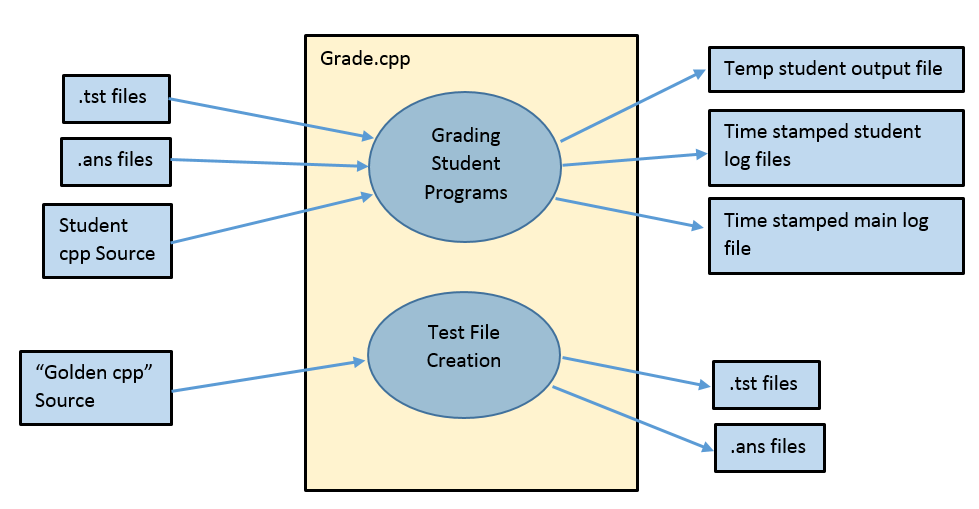
\includegraphics[width=0.75\textwidth]{./Arch_generic}
\end{center}
\caption{Architecture Diagram for the Tester Application \label{arch_generic}}
\end{figure}


\subsection{Data Flow Diagram} 
%See Figure~\ref{dataflow}.

\begin{figure}[H]
\begin{center}
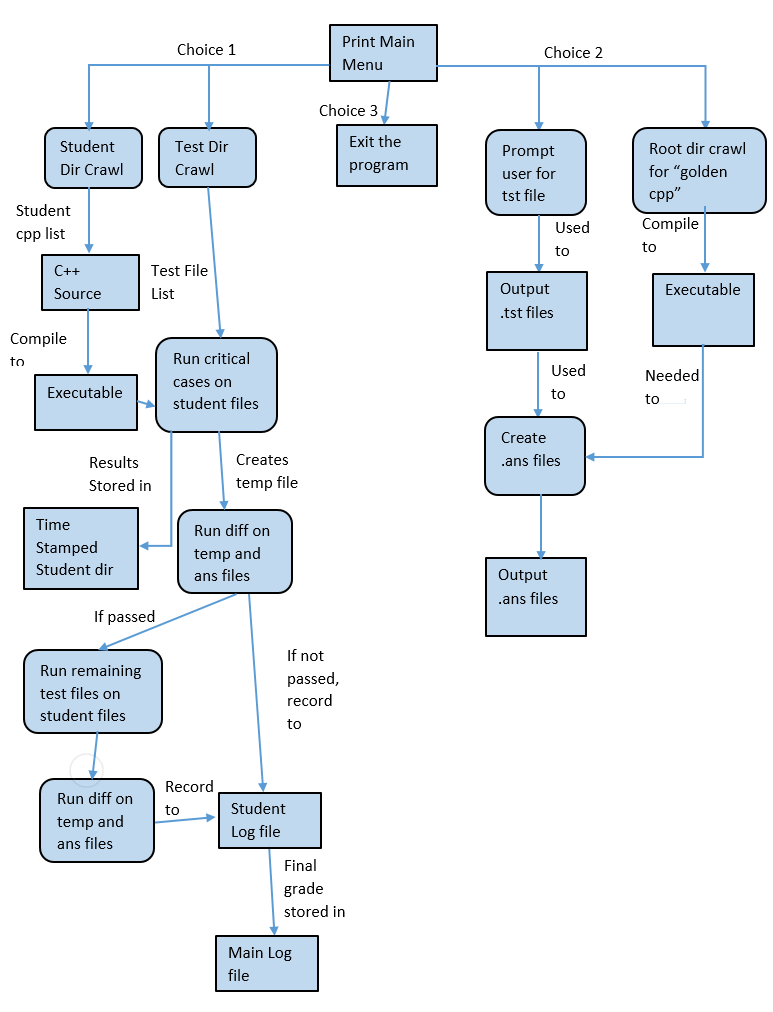
\includegraphics[width=0.9\textwidth]{./Dataflow}
\end{center}
\caption{ Data Flow Diagram for the Tester Application \label{dataflow}}
\end{figure}


\subsection{Design Details}
The following function does the directory crawl and stores the relative path to 
 .tst file in the "dest" vector which is passed by reference. This is the recursive function that searches all sub-directories of the directory root which contains the executable program:
\begin{lstlisting}
void directoryCrawl( bool type, string dir, string file, bool recursive, 
							vector <string> &names, bool critFLAG )
{
    // Structure in dirent.h stores the file name and the file id number
    struct dirent **namelist;

    int n;
    int i;

    n = scandir(dir.c_str(), &namelist, 0, alphasort);

    if(n == -1)
        return;


    for ( i = 2; i < n; i++ )
    {
        string tempFile = namelist[i]-> d_name;

        if(string::npos != tempFile.find(file))
        {
            if( DT_DIR == namelist[i] -> d_type && type == DIRECTORIES )
            {
                names.push_back(dir + "/" + tempFile);
                //cout << dir << "/" << tempFile << endl;
            }
            if( DT_REG == namelist[i] -> d_type && type == FILES )
            {
                if ( string::npos != tempFile.find("_crit.tst") && !critFLAG )
                    continue;

                names.push_back(dir + "/" + tempFile);
                //cout << dir << "/" << tempFile << endl;
            }
        }

        if (recursive && DT_DIR == namelist[i] -> d_type && 
        			tempFile != "." && tempFile != ".." )
            directoryCrawl( type, dir + "/" + tempFile, file, 
            				true , names, critFLAG );

    }


    for(i = 0; i < n; i++)
        delete []namelist[i];
    delete []namelist;
}
\end{lstlisting}
Once this function has finished executing the destination vector contains a listing of all paths to .tst files to be run by the program being tested.



\section{Test Single Program Against Found Test Cases}

\subsection{Technologies  Used}
The only technology used in this section is C++ code.

\subsection{Component  Overview}
The purpose for this section is to compile the C++ code, loop through the list of .tst files in the directory, and check if the program output matches the .ans file output.

\subsection{Phase Overview}
Testing a program against located test cases is necessary in the second and third phases because we must be able to check the program's output against the .ans file to see if each test was a success or failure before program output can be prepared.

\subsection{ Architecture  Diagram}
Due to the small size of the application, a single diagram describing the architecture of the program is provided in Figure~\ref{arch_generic}

\subsection{Data Flow Diagram}
Due to the small size of the application, a single diagram describing the data flow for the program is provided in Figure~\ref{dataflow}.


\subsection{Design Details}
Testing the program may be broken down into three sections:
\begin{itemize}
	\item Compiling source C++ code
	\item Running C++ code against test case
	\item Determining if program output was correct for test case
\end{itemize}
The following function compiles the program using a system call to g++:
\begin{lstlisting}
bool compile_code( string filename ){

    // Strip off the .cpp extension
    string executable = removeExtension( filename );
    
    // Produce "g++ program.cpp -o program" command
    string compile_instruction = "g++ ";
    compile_instruction += filename;
    compile_instruction += " -o ";
    compile_instruction += executable; // name of golden cpp file

    // Compile the source code
    system( compile_instruction.c_str() );

    return true;
}
\end{lstlisting}
To run the executable against a test case another system call is made redirecting input from the test file and output. Once the program has been run, a system "diff" is done on the output file versus the answer file:
\begin{lstlisting}
bool test(const string &program, string a_file, string tst_file)
{

    //runs the .cpp program with redirected input and output
    system(string(program + " < " + tst_file + " > " + a_file).c_str());

    //runs a diff command on the .ans and .out files and returns true if 
    //they are not different
    if(system(string("diff " + a_file + " " 
    					 + tst_file.substr(0,tst_file.find_last_of('.') )
    					 + ".ans").c_str()) == 0)
    {
        return true;
    }

    return false;
}
\end{lstlisting}

\section{Record and Summarize Test Results }

\subsection{Technologies  Used}
The only technology used in this section is C++ code.

\subsection{Component  Overview}
After the test cases have been run a timestamped .log file needs to be produced. It should include if each test case passed or failed as well as the percentage of correct files along with the total number of correct and incorrect test cases.

\subsection{Phase Overview}
This component is included in the fourth phase of production. It was done last because the full output file could not be produced without knowing the results of all the test cases.

\subsection{ Architecture  Diagram}
Due to the small size of the application, a single diagram describing the architecture of the program is provided in Figure~\ref{arch_generic}


\subsection{Data Flow Diagram}
Due to the small size of the application, a single diagram describing the data flow for the program is provided in Figure~\ref{dataflow}.

\subsection{Design Details}
The formatted output is produced by the outputLogFile() function. It lists if each test case was a pass or failure along with overall test statistics. 



\section{Run Test Cases on Entire Class}

\subsection{Technologies  Used}
The only technology used in this section is C++ code.

\subsection{Component  Overview}
It is often useful to run a batch of student files over the test files. For example, when grading an entire class assignment, there are many students to grade. 

\subsection{Phase Overview}
This feature is released in the second phase (corresponding to the second sprint). It is a major product feature and must be included in this phase.

\subsection{Architecture Diagram}
Due to the small size of the application, a single diagram describing the architecture of the program is provided in Figure~\ref{arch_generic}


\subsection{Data Flow Diagram}
Due to the small size of the application, a single diagram describing the data flow for the program is provided in Figure~\ref{dataflow}.

\subsection{Design Details}
To run all student files against all test files, two loops are used (the first to loop over students, the second over test cases). The main function for testing is called "grade". It includes the loops and makes calls to the previously described functions to compile and run the code grades all student files. Pseudocode for this function is:
\begin{lstlisting}
void grade( vector <string> critTestCases, vector <string> testCases,
            vector <string> studentDirs, ofstream &LOG, string exeTime )
{
    string program;
    vector<string>::iterator stdnt_it;
    vector<string>::iterator test_it;
    vector<string> cppFiles;
    bool FLAG;
    int passCount;
    int currCount;
    ofstream student_LOG;

	//Loop through student directories
    for ( stdnt_it = studentDirs.begin(); stdnt_it < studentDirs.end(); 
    		stdnt_it++)
    {
        //Find test files
        directoryCrawl( FILES, *stdnt_it, ".cpp", false, cppFiles, 0 );

		//If we found a cpp file, check if directory name == cpp name
        if (cppFiles.size() > 0)
        {
            executable = fileNameFromPath(cppFiles[0]);
            executable = removeExtension(executable);
            if (dir_name != executable)
            {
                continue;
            }
        }
        else
        {
            continue;
        }
		// Compile the student's executable
        compile_code(cppFiles[0]);

        // Run each critical test on the student's code
        for ( test_it = critTestCases.begin(); \\
        		test_it != critTestCases.end() && FLAG == true; test_it++ )
        {
            //Get the output file name
            //Output file name to student log file
            if ( !test(executable,out_file,*test_it) )
                //Log a failure if failed critical test cases
            else
                //Log the student as a pass for critical cases
        }
		//If student passed the critical cases
        if ( FLAG == true)
            student_LOG << endl << "Non-Critical Test Cases:" << endl << endl;

		// If student passed critical cases, run other test cases
        for ( test_it = testCases.begin(); test_it != testCases.end() 
        		&& FLAG == true; test_it++ )
        {
            //Get the input and log file names
            //If the student passes a test case
            if ( test(executable,out_file, *test_it) )
            {
                //Increment passes, log to student file
            }
            else
                //Log a failed test case
        }
        //If student passed critical cases, output percent to log file
        if ( FLAG == true )
        {
            //Output to main log file
            LOG << stdnt_it -> substr( stdnt_it -> find_last_of('/') + 1, 
            		stdnt_it -> length() ) << ": " 
            		<< calc_percentage( passCount, testCases.size() ) << endl;
        }
        if ( FLAG )
        {
            // Output the passes, fails and percentages 
            //  to the student's log file.
        }

        student_LOG.close();
    }
}
\end{lstlisting}

\section{Run Critical Test Cases First}

\subsection{Technologies  Used}
The only technology used in this section is C++ code.

\subsection{Component  Overview}
To prevent running student programs which have failed the basic 
requirements it is useful to have "critical test cases" which test
the program's basic functionality. These test files are run first and, 
if failed, no not permit further testing on the student's program.

\subsection{Phase Overview}
This component is done in the second phase of production for the second
release.

\subsection{ Architecture  Diagram}
Due to the small size of the application, a single diagram describing
the architecture of the program is provided in Figure~\ref{arch_generic}


\subsection{Data Flow Diagram}
Due to the small size of the application, a single diagram
describing the data flow for the program is provided in Figure~\ref{dataflow}.

\subsection{Design Details}
In order for critical files to be tested first, a directory crawl searching for
"crit" files is performed. After getting critical test files the program is run
one by one against them. If the program fails a critical test case then the grade
is recorded as a failure and no more testing is done. If all critical test cases
are passed the program continues to test the student program to get a percentage
grade as opposed to "FAILED" as is outputted on an incorrect critical test case.

Below is the code snippet (taken from the grade function) that runs critical test
cases:

\begin{lstlisting}
//critTestCases contains a list of critical test cases
// The critical case directory crawl is done in main and
// passed as a parameter
for ( test_it = critTestCases.begin(); test_it != critTestCases.end() 
		&& FLAG == true; test_it++ )
        {
            string testFile = fileNameFromPath(*test_it);
            string out_file = *stdnt_it + "/" + testFile;
            out_file = removeExtension(out_file);
            out_file += ".out";

            currCount++;
            student_LOG << string( removeExtension(testFile) ) << ": ";

            if ( !test(executable,out_file,*test_it) )
            {
                LOG << stdnt_it -> substr( stdnt_it -> find_last_of('/') + 1,
                			 stdnt_it -> length() ) << ": FAILED" << endl;
                FLAG = false;
                student_LOG << "FAIL" << endl << endl;

                student_LOG << "Student Failed a Critical Test File" << endl;


            }
            else
                student_LOG << "PASS" << endl;
        }
\end{lstlisting}

 
\section{Generate Test Cases and Corresponding Answer Files}

\subsection{Technologies  Used}
The only technology used in this section is C++ code.

\subsection{Component  Overview}
The testing program has the ability to generate test case files
automatically using specifications provided by the user. After 
generating the test file a "Golden CPP" (a correct solution to
the program) is compiled and run against the test case to generate
a corresponding answer file

\subsection{Phase Overview}
This component is done in the second phase of production. It was not
needed to get the first version of the testing program and has been
included here.

\subsection{ Architecture  Diagram}
Due to the small size of the application, a single diagram describing the architecture of the program is provided in Figure~\ref{arch_generic}


\subsection{Data Flow Diagram}
Due to the small size of the application, a single diagram describing the data flow for the program is provided in Figure~\ref{dataflow}.

\subsection{Design Details}
When creating test cases the user specifies how many test files, how many entries per test file, float or integer values, a range on test file entry values, and the name of the test files to be generated. A random number generator will then determine the the number of entries ($l$, from zero to the max size specified by the user) and generate a test file with $l$ entries within the range. File output will either contain floating point or integer values, depending on what was specified by the user. The basic algorithm is provided below, but the source code is provided in grade.cpp.

\begin{lstlisting}
//Generate test cases and answer files 
bool create_test_cases()
{
    // Find how many test files the user wants to create

    // Enter how many entries will be in the test file
    
    // Prompt for (i)nts or (f)loats

    // Get a minimum for the range if the user wants to supply it

    // Get a maximum for the range if the user wants to supply it

    // Prompt for a test file name if the user wants to supply it

    // Crawl through the root directory to find the golden cpp
    
    // Since our grade.cpp file could possibly be in the base directory
    // try to remove it from the list, just in case...

    
    // The "golden cpp" will be the only item left in the list since it 
    // is the only .cpp file in the root directory. Compile it now!

    // For each test file that we need to create
    for( int j=0; j < num_cases; j++  ){
        
        // Assume the file hasn't opened

        //Piece together the path to store the tst and ans files
        
        // Open the file to write

        // Abort this single test file if we couldn't open it to write
 
        // If we opened the test file then fill it with randoms within the
        // user supplied range
       
        // Close the test file

        // Using the newly generated test file, generate the answer file
        
    }

}
\end{lstlisting}

Once the test file is created the Golden CPP is compiled and run against the test case. This generates the corresponding answer file for student programs to be compared against. This is done in create\_ans\_file() which is provided below:

\begin{lstlisting}
//Generate an answer file for a newly created test file using the golden cpp
bool create_ans_file( string test_file_path, string golden ){

    // Remove the .cpp file extension
    string executable = removeExtension( golden );

    // Append .ans file extension 
    string ans_file_path = test_file_path;
    ans_file_path = ans_file_path.replace( ans_file_path.find( ".tst" ), 4, ".ans" );

    // Piece together the shell command to run the program
    // with redirected input and output
    string run_instruction = "./";
    run_instruction += executable; 
    run_instruction += " < ";
    run_instruction += test_file_path;
    run_instruction += " > ";
    run_instruction += ans_file_path;

    // Run the command
    system( run_instruction.c_str() );
    return true;
}
\end{lstlisting}

